\chapter{Introduction}
\label{introduction}

%intro to the intro here


\section{Motivation}

%expanded version of the above? need stats on depression and schizophrenia
It is estimated that disorders of the brain cost Europe €798 billion Euros in 2010\autocite{olesen_economic_2012}.
Specifically, depression is estimated to cost Europe €91.9 billion in 2004 and schizophrenia along with associated psychotic disorders is estimated at €93.9 billion.
There are many diseases with currently limited treatment options in the brain, and a deeper understanding of the brain is required to treat them.

These diseases are very likely to act at the synaptic level\autocites{chua_architecture_2010,synsys}.
However, the exact proteins or genes involved in these diseases are unknown.
If it is possible to even gain slightly more information about associated proteins at the synapse it may be possible to develop new treatments\autocite{li_interaction_2010}.

In addition, as a project this includes work from various areas, such as Bioinformatics, Machine Learning and Software Development that made it a good learning exercise.
It is a worthwhile investment in the fundamentals of constructing PPI networks.

%overview of the project or the report? pretty sure it's the report
\section{Outline}
%sections to cover:
% background
% methods
% results
% conclusion

This project involved combining both direct and indirect data sources to create weighted edges in a PPI graph to affect the communities detected by a Community Detection algorithm.
A flow chart describing this process and the elements involved is shown in figure \ref{fig:expflow}.
There are three main input sources shown, the pull-down experiments, direct data and indirect data.
Pull-down experiments were used to identify the proteins of interest, which were used to build an interaction network using direct data sources, such as interaction databases.
The indirect data sources, such as functional annotations of proteins, were used along with direct data sources in the process to generate weighted graphs.

%flow charts from the proposal could go here
\begin{figure}
    \centering
    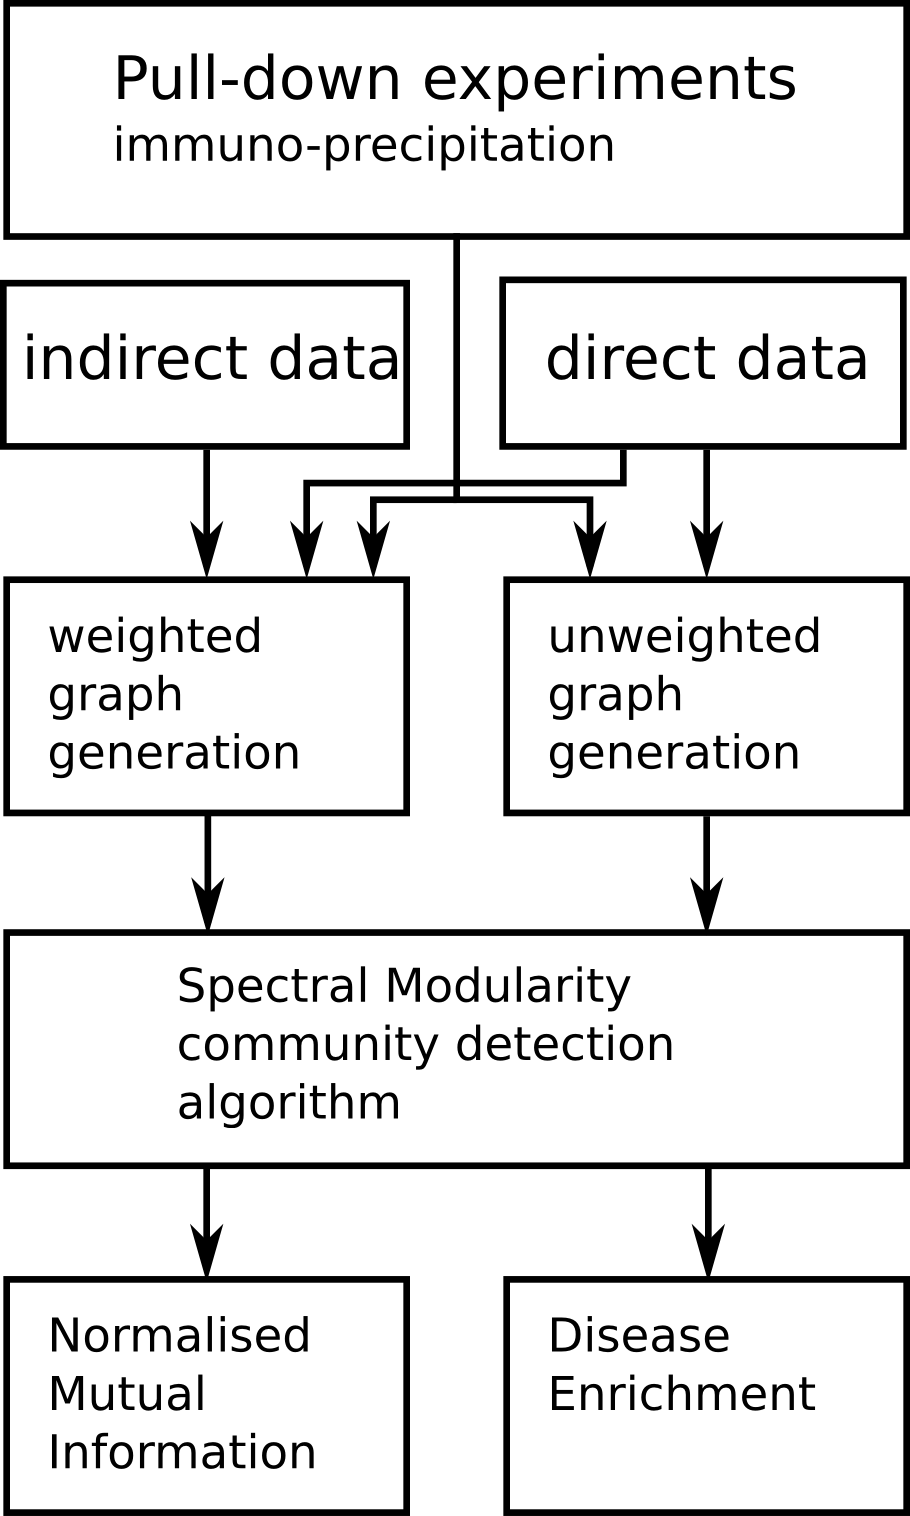
\includegraphics{expflow.png}
    \caption{A flow chart describing how the elements of the project as a whole, as shown in the project proposal.}
    \label{fig:expflow}
\end{figure}

The resulting weighted and unweighted PPI graphs were then separated into communities using a Community Detection algorithm.
These communities could then be compared using the two methods named in figure \ref{fig:expflow}: Disease Enrichment and NMI.
Results of these tests were the final deliverable of the project.

%information about the repository, organisation of project files etc
\subsection{Repository}

%about using git as version control online, anything I can reference here?
Git is version control software and was used extensively in this project in combination with Github\autocite{github} and git-annex\autocite{gitannex}.
The project is built from two repositories, the first inside the second: a large git-annex based repository containing all the data and a smaller git repository stored on github containing all the code and documentation for the report\autocite{opencast-bio}.
History for all the code and documentation, every previous version, is available publicly online but the data cannot be made publicly available.

%metrics describing the repository
Hosting the code online was intended to aid remote collaborators.
It is also useful in order to maintain an accurate log of the work involved in the project.
The repository also includes a wiki\autocite{opencastbiowiki} providing documentation on some of the code available in the repository and weekly reports covering the entire project.

%structure of the repository
The repository consists of several directories:

\begin{itemize}
    \item notebooks:
        \begin{itemize}
            \item Contains IPython notebooks covering code executed during the project.
            \item Each notebook includes inline documentation on what is being done, and why.
        \end{itemize}
    \item ocbio:
        \begin{itemize}
            \item This contains the Python module of code developed during the project.
            \item The major component of this is the extract.py file, which deals with writing feature vectors for use in classification.
        \end{itemize}
    \item proposal:
        \begin{itemize}
            \item Only contains the original proposal for the project.
        \end{itemize}
    \item report:
        \begin{itemize}
            \item Contains this report and all the required files to compile it.
            \item Based on a repository for Masters project templates\autocite{ug4template} with modifications by Danilo Orlando.
        \end{itemize}
    \item scripts:
        \begin{itemize}
            \item Contains scripts, but these were not used during the bulk of the project.
        \end{itemize}
\end{itemize}

%future usefulness?
The code in this repository may be useful to a future project, but could also be substantially improved upon.
It is more likely that the notes on how to go about a protein interaction prediction task, and this report, will be more useful to future work.

%planning and time management
\section{Planning}

The project was split between five tasks:

\begin{itemize}
    \item Feature Extraction
    \item Classifier Training
    \item Community Detection and analysis
    \item Writing the report
\end{itemize}

The original plan for this project placed feature extraction as the dominant task.
This was correct, in that the project only found time for training the classifier and performing Community Detection within the last five weeks.
However, the reasons for delays were unknown at the time of beginning and were due largely to inexperience with Bioinformatics.

%mention weekly reports
Weekly reports were kept as a summary of the work completed every week for supervisors and to maintain a log of the project.
These can be found on the project wiki\autocite{opencastbiowiki}.

%progress flow charts from the proposal could go here, or above

%could also include one updated to reflect the real project

%should also mention the prototype run through and which week it occurred in 

\section*{Conclusion}

The following report covers the background information necessary to understand the methods of the project and the results which were obtained.
It was approached as an opportunity to use a variety of new tools, and each will be described as the report continues.
